\documentclass[../../../../main.tex]{subfiles}
\begin{document}

図のように底面の半径1，上面の半径 $1-x$，高さ $4x$ の直円すい台 $A$ と，
底面の半径 $\displaystyle1-\frac{x}{2}$，上面の半径 $\displaystyle\frac{1}{2}$，高さ $1-x$ の直円すい台 $B$ がある．
ただし，$0 \leqq x \leqq 1$ である．
$A$ と $B$ の体積の和を $V(x)$ とするとき，$V(x)$ の最大値を求めよ．

\begin{figure}[htbp]
  \centering
  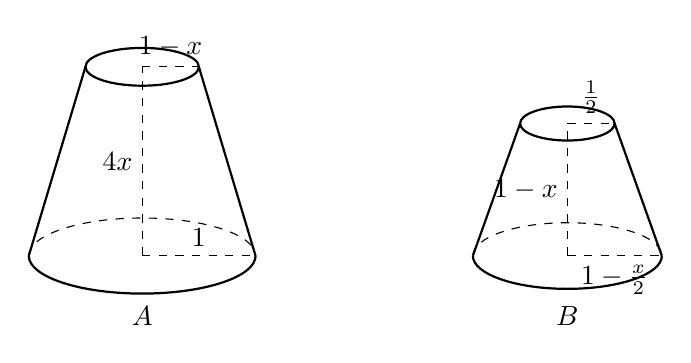
\begin{tikzpicture}[scale=1.2, >=stealth]
    % 直円すい台 A
    \begin{scope}[shift={(0,0)}]
      \draw[thick] (-1.2,0) arc (180:360:1.2 and 0.4);
      \draw[dashed] (-1.2,0) arc (180:0:1.2 and 0.4);

      \draw[thick] (0, 2.0) ellipse (0.6 and 0.2);

      \draw[thick] (-1.2,0) -- (-0.6, 2.0);
      \draw[thick] (1.2,0) -- (0.6, 2.0);

      \draw[dashed] (0,0) -- (0,2.0) node[midway, left] {$4x$};
      \draw[dashed] (0,2.0) -- (0.6,2.0) node[midway, above] {$1-x$};
      \draw[dashed] (0,0) -- (1.2,0) node[midway, above] {$1$};

      \node[below=15pt] at (0,0) {$A$};
    \end{scope}

    % 直円すい台 B
    \begin{scope}[shift={(4.5,0)}]
      \draw[thick] (-1.0,0) arc (180:360:1.0 and 0.35);
      \draw[dashed] (-1.0,0) arc (180:0:1.0 and 0.35);

      \draw[thick] (0, 1.4) ellipse (0.5 and 0.18);

      \draw[thick] (-1.0,0) -- (-0.5, 1.4);
      \draw[thick] (1.0,0) -- (0.5, 1.4);

      \draw[dashed] (0,0) -- (0,1.4) node[midway, left] {$1-x$};
      \draw[dashed] (0,1.4) -- (0.5,1.4) node[midway, above] {$\frac{1}{2}$};
      \draw[dashed] (0,0) -- (1.0,0) node[midway, below] {$1-\frac{x}{2}$};

      \node[below=15pt] at (0,0) {$B$};
    \end{scope}
  \end{tikzpicture}
\end{figure}

\end{document}
